\chapter{Data acquisition}

The data used in the paper has been gathered over the course of three months, starting in early March and ending in late May. The data has been obtained with the help of three student volunteers. Each volunteer carried a phone, provided by TODO. The phones are Samsung Galaxy Nexus and are running the Android operating system \cite{android}. 

Each phone came with two apps. The first recorded regularly a multitude of information, such as bluetooth RSSI, GPS traces, battery usage and cell tower information \cite{Stopczynski}, while the second allowed the volunteers to manually name the person they are in physical proximity with. 

This gave rise to two types of data. First, a continuous stream of regular measurements from the first app, and punctual messages from the second app. Below we will go into more detail about how exactly the two types of data look, how are they gathered and finally, how the two are combined to create a unitary set which serves as a basis for the machine learning algorithms.

\section{FriendFinder app}

\subsection{App overview and implementation}

As the app is made for the Android operating system, it is implemented using Java for Android \cite{jandroid}. It has a Google App Engine backend \cite{googleapp}. Fig \ref{pic:ff_prtscr} shows the app. 

\begin{figure}[h]
	\begin{center}
		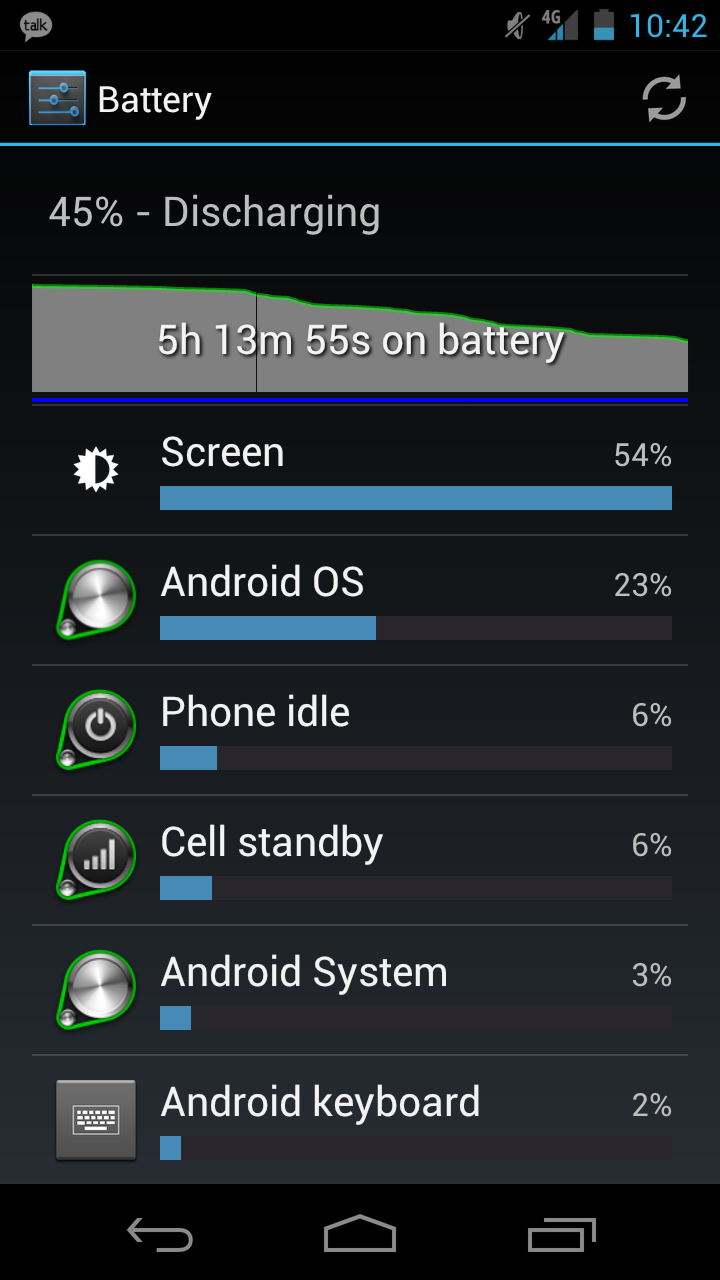
\includegraphics[scale=0.2]{figures/galaxy-nexus-battery.png}
	\end{center}
	
	\caption{FriendFinder app}.
	\label{pic:ff_prtscr}

\end{figure} 

FriendFinder is implemented using a client server architecture, where the clients are the apps installed on the phone, and the server is the Google App Engine. Fig \ref{pic:clientserver} shows an overview of this particular architecture.

\begin{figure}[h]
	\begin{center}
		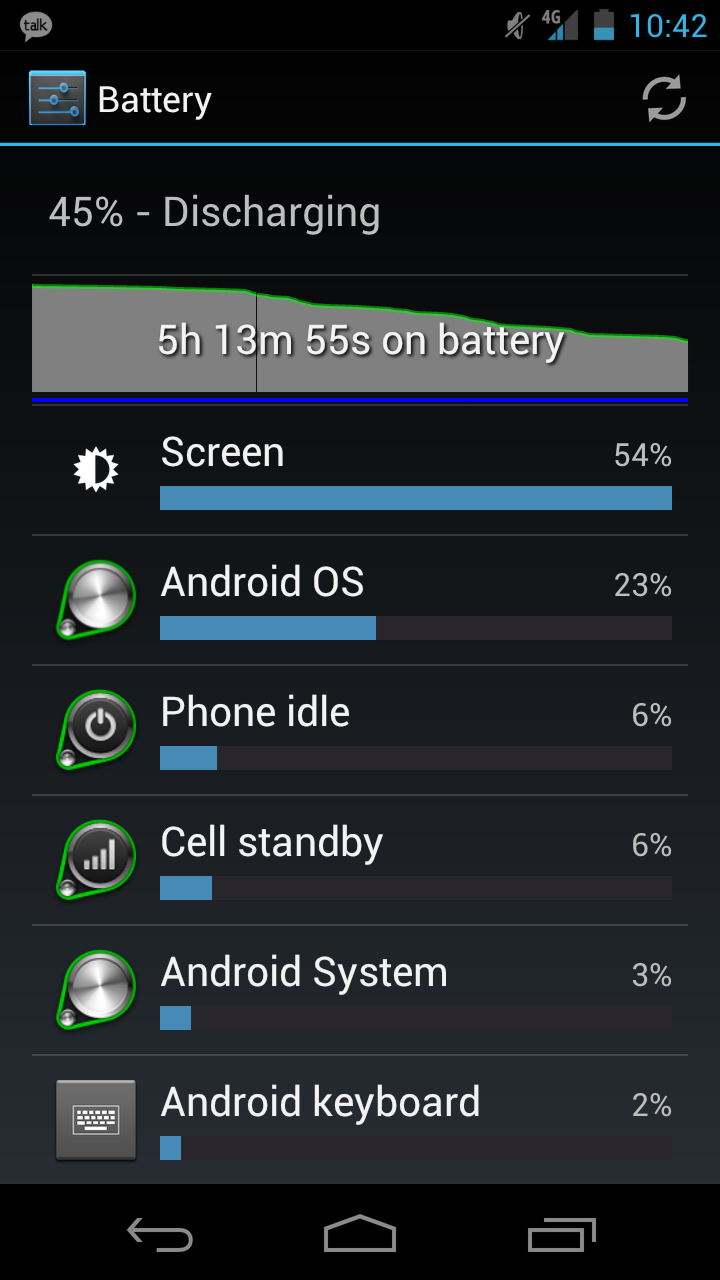
\includegraphics[scale=0.2]{figures/galaxy-nexus-battery.png}
	\end{center}
	
	\caption{FriendFinder app}.
	\label{pic:clientserver}

\end{figure} 

\subsection{Data}


\section{SensibleDTU data} 	